\chapter[The Tooth Thrall]{
    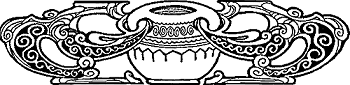
\includegraphics[width=9.3cm]{viking-tales/012}\\
    The Tooth Thrall}

\lettrine{W}{hen} Harald was seven months old he cut his first tooth.
Then his father said:
\vskip\baselineskip
``All the young of my herds, lambs and calves and colts, that have been
born since this baby was born I this day give to him. I also give to him
this thrall, Olaf. These are my tooth-gifts to my son.''

The boy grew fast, for as soon as he could walk about he was out of
doors most of the time. He ran in the woods and climbed the hills and
waded in the creek. He was much with his tooth thrall, for the king had
said to Olaf:

``Be ever at his call.''

Now this Olaf was full of stories, and Harald liked to hear them.

``Come out to Aegir's Rock, Olaf, and tell me stories,'' he said almost
every day.

So they started off across the hills. The man wore a long, loose coat of
white wool, belted at the waist with a strap. He had on coarse shoes and
leather leggings. Around his neck was an iron collar welded together so
that it could not come off. On it were strange marks, called runes, that
said:

``Olaf, thrall of Halfdan.''

But Harald's clothes were gay. A cape of gray velvet hung from his
shoulders. It was fastened over his breast with great gold buckles. When
it waved in the wind, a scarlet lining flashed out, and the bottom of a
little scarlet jacket showed. His feet and legs were covered with gray
woolen tights. Gold lacings wound around his legs from his shoes to his
knees. A band of gold held down his long, yellow hair.

It was a wild country that these two were walking over. They were
climbing steep, rough hills. Some of them seemed made all of rock, with
a little earth lying in spots. Great rocks hung out from them, with
trees growing in their cracks. Some big pieces had broken off and rolled
down the hill.

``Thor broke them,'' Olaf said. ``He rides through the sky and hurls his
hammer at clouds and at mountains. That makes the thunder and the
lightning and cracks the hills. His hammer never misses its aim, and it
always comes back to his hand and is eager to go again.''

When they reached the top of the hill they looked back. Far below was a
soft, green valley. In front of it the sea came up into the land and
made a fiord. On each side of the fiord high walls of rock stood up and
made the water black with shadow. All around the valley were high hills
with dark pines on them. Far off were the mountains. In the valley were
Halfdan's houses around their square yard.

``How little our houses look down there!'' Harald said. ``But I can
almost--yes, I can see the red dragon on the roof of the feast hall. Do
you remember when I climbed up and sat on his head, Olaf?''

He laughed and kicked his heels and ran on.

\begin{figure}[ht]
    \centering
    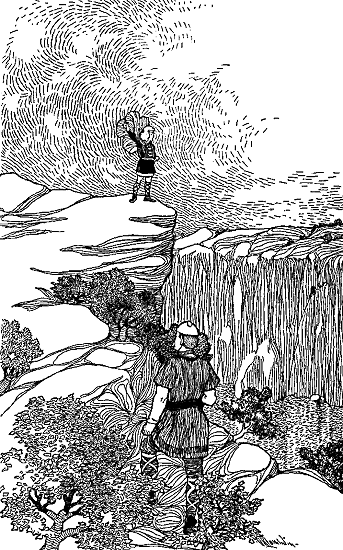
\includegraphics[width=9.1cm]{viking-tales/013}
    \caption{
        ``He threw back his cape and drew a little dagger from his
        belt''}
\end{figure}

At last they came to Aegir's Rock and walked up on its flat top. Harald
went to the edge and looked over. A ragged wall of rock reached down,
and two hundred feet below was the black water of the fiord. Olaf
watched him for a while, then he said:

``No whitening of your cheek, Harald? Good! A boy that can face the fall
of Aegir's Rock will not be afraid to face the war flash when he is a
man.''

``Ho, I am not afraid of the war flash now,'' cried Harald.

He threw back his cape and drew a little dagger from his belt.

``See!'' he cried; ``does this not flash like a sword? And I am not
afraid. But after all, this is a baby thing! When I am eight years old I
will have a sword, a sharp tooth of war.''

He swung his dagger as though it were a long sword. Then he ran and sat
on a rock by Olaf.

``Why is this Aegir's Rock?'' he asked.

``You know that Asgard is up in the sky,'' Olaf said. ``It is a wonderful
city where the golden houses of the gods are in the golden grove. A high
wall runs all around it. In the house of Odin, the All-father, there is
a great feast hall larger than the whole earth. Its name is Valhalla. It
has five hundred doors. The rafters are spears. The roof is thatched
with shields. Armor lies on the benches. In the high seat sits Odin, a
golden helmet on his head, a spear in his hand. Two wolves lie at his
feet. At his right hand and his left sit all the gods and goddesses, and
around the hall sit thousands and thousands of men, all the brave ones
that have ever died.

``Now it is good to be in Valhalla; for there is mead there better than
men can brew, and it never runs out. And there are skalds that sing
wonderful songs that men never heard. And before the doors of Valhalla
is a great meadow where the warriors fight every day and get glorious
and sweet wounds and give many. And all night they feast, and their
wounds heal. But none may go to Valhalla except warriors that have died
bravely in battle. Men who die from sickness go with women and children
and cowards to Niflheim. There Hela, who is queen, always sneers at
them, and a terrible cold takes hold of their bones, and they sit down
and freeze.

``Years ago Aegir was a great warrior. Aegir the Big-handed, they called
him. In many a battle his sword had sung, and he had sent many warriors
to Valhalla. Many swords had bit into his flesh and left marks there,
but never a one had struck him to death. So his hair grew white and his
arms thin. There was peace in that country then, and Aegir sorrowed,
saying:

`\,``I am old. Battles are still. Must I die in bed like a woman? Shall I
not see Valhalla?'

``Now thus did Odin say long ago:

`\,``If a man is old and is come near death and cannot die in fight, let
him find death in some brave way and he shall feast with me in
Valhalla.'

``So one day Aegir came to this rock.

`\,``A deed to win Valhalla!' he cried.

``Then he drew his sword and flashed it over his head and held his
shield high above him, and leaped out into the air and died in the water
of the fiord.''

``Ho!'' cried Harald, jumping to his feet. ``I think that Odin stood up
before his high seat and welcomed that man gladly when he walked through
the door of Valhalla.''

``So the songs say,'' replied Olaf, ``for skalds still sing of that deed
all over Norway.''

\begin{figure}[hb]
    \centering
    \vskip8pt
    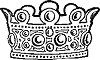
\includegraphics[width=2.7cm]{viking-tales/014}
\end{figure}
